\input format.tex
\input defs.tex

%% begin presentation

\title{\large \bfseries Distributed Deep Q-Learning}

\author{Hao Yi Ong, Kevin Chavez, and Augustus Hong\\[3ex]
CME 323, Stanford University}

\date{June 3, 2015}

\begin{document}

\frame{
\thispagestyle{empty}
\titlepage
}

\section{Introduction}

\begin{frame}{Motivation}
  \begin{itemize}\itemsep=12pt
  
    \item long-standing challenge of RL
    \vspace*{0.5em}
    \begin{itemize}
        \item control with high-dimensional sensory inputs (\eg, vision, speech)
        \item shift away from reliance on hand-crafted features
    \end{itemize}
    
    \item utilize breakthroughs in deep learning for RL
    \vspace*{0.5em}
    \begin{itemize}
        \item extract high-level features from raw sensory data
        \item learn better representations than handcrafted features with neural network architectures used in supervised and unsupervised learning
        \item train efficiently with stochastic gradient descent
    \end{itemize}

  \end{itemize}
\end{frame}

\begin{frame}{Playing Atari}
    \begin{figure}
        \centering
        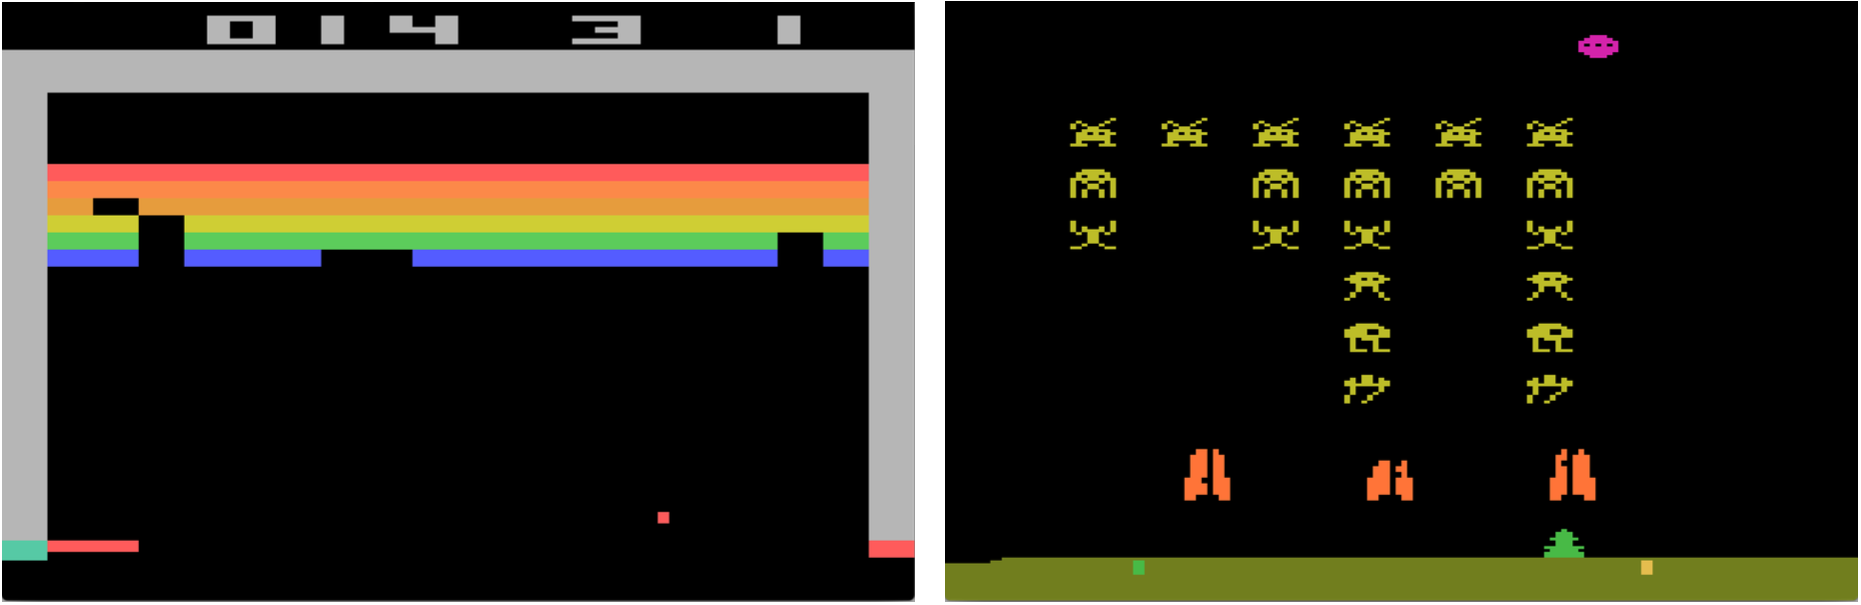
\includegraphics[width=0.8\textwidth]{atari-ex1.png}
    \end{figure}
    \begin{figure}
        \centering
        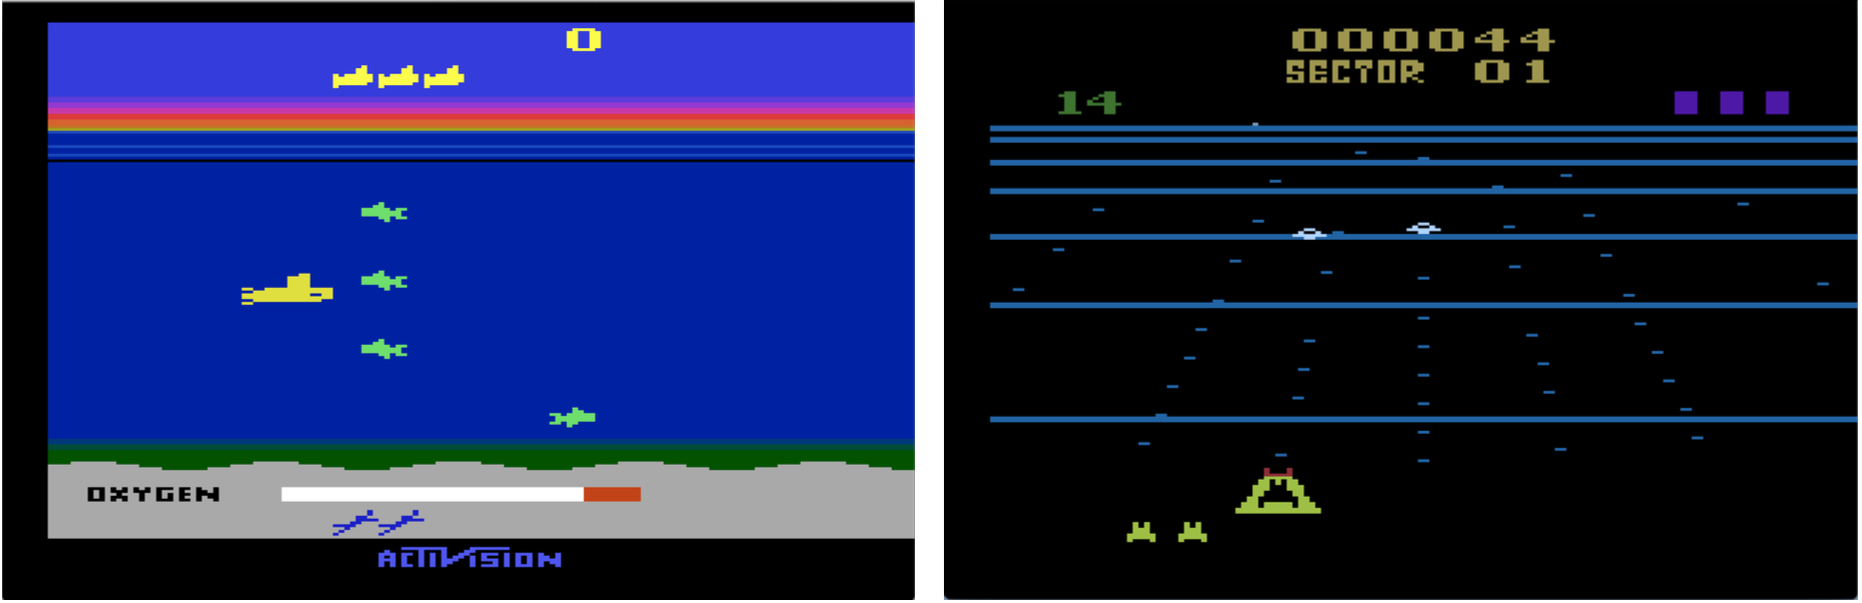
\includegraphics[width=0.8\textwidth]{atari-ex2.png}
    \end{figure}
\end{frame}

\begin{frame}{Deep reinforcement learning}
    \begin{itemize}\itemsep=12pt

        \item connecting RL with deep neural networks
        \vspace*{0.5em}
        \begin{itemize}
            \item reinforcement learning approach to obtain control policies
            \item use high-dimensional sensory input
        \end{itemize}

        \item practical considerations
        \vspace*{0.5em}
        \begin{itemize}
            \item differences between supervised/unsupervised deep learning and RL
            \item algorithm must learn like a human player
        \end{itemize}

    \end{itemize}
\end{frame}

\begin{frame}{Theoretical complications}
    \begin{itemize}\itemsep=12pt

        \item deep learning usually requires huge hand-labeled training datasets
        \vspace*{0.5em}
        \begin{itemize}
            \item sparse, noisy, and delayed reward signal in RL
            \item delay of $\sim10^{3}$ time steps between actions and resulting rewards
            \item \cf\ direct association between inputs and targets in supervised learning
        \end{itemize}

    \end{itemize}
\end{frame}

\begin{frame}{Theoretical complications}
    most deep learning algorithms assume
    \vspace*{0.5em}
    \begin{itemize}\itemsep=12pt

        \item independence between data samples
        \vspace*{0.5em}
        \begin{itemize}
            \item sequences of highly correlated states in RL problems
        \end{itemize}

        \item fixed underlying data distribution
        \vspace*{0.5em}
        \begin{itemize}
            \item distribution changes as RL algorithm learns new behaviors
        \end{itemize}

    \end{itemize}
\end{frame}

\begin{frame}{Emulating human learning}
    \begin{itemize}\itemsep=12pt
        
        \item neural network not provided
        \vspace*{0.5em}
        \begin{itemize}
            \item game-specific information
            \item hand-designed visual features
            \item internal state of emulator
        \end{itemize}

        \item generalizing across games with the same
        \vspace*{0.5em}
        \begin{itemize}
            \item network architecture
            \item training algorithm hyperparameters
        \end{itemize}

    \end{itemize}
\end{frame}

\begin{frame}{Goals}
    first deep RL model
    \vspace*{0.5em}
    \begin{itemize}\itemsep=12pt
        
        \item single game-agnostic, robust neural network agent
        \vspace*{0.5em}
        \begin{itemize}
            \item must succeed in various Atari test problems
        \end{itemize}

        \item control policies with high-dimensional sensory input
        \vspace*{0.5em}
        \begin{itemize}
            \item obtain better internal representations than handcrafted features
        \end{itemize}

        \item fast training algorithm
        \vspace*{0.5em}
        \begin{itemize}
            \item efficiently produce, use, and process training data
        \end{itemize}

    \end{itemize}
\end{frame}

\begin{frame}{Prior work}
    TD-gammon \cite{Tes:95}
    \vspace*{0.5em}
    \begin{itemize}\itemsep=12pt

        \item backgammon-playing program learned by RL and self-play

        \item model-free RL algorithm similar to Q-learning

        \item approximated state value function with multilayer perceptron with one hidden layer

        \item fared poorly in chess, Go, and checkers
        
    \end{itemize}
\end{frame}

\begin{frame}{Prior work}
    neural fitted Q-learning \cite{Rie:05}
    \vspace*{0.5em}
    \begin{itemize}\itemsep=12pt

        \item minimizes sequence of loss functions ($\ell_{2}$-norm)
    
        \item success with purely visual input by first using deep autoencoders to learn reduced task representation
    
        \item most similar to current paper
    
    \end{itemize}
\end{frame}

\begin{frame}{Prior work}
    other works include
    \vspace*{0.5em}
    \begin{itemize}\itemsep=12pt

        \item Q-learning with experience replay, simple neural network, and reduced visual inputs \cite{Lin:93}

        \item restricted Boltzmann machines as value function or policy approximators \cite{SH:04,HST:12}

        \item evolutionary architecture used to evolve separate neural networks representing strategies for different games \cite{HMS:13}

    \end{itemize}
\end{frame}

\section{Mathematical formulation}

\begin{frame}{Playing Atari}
    \begin{figure}
        \centering
        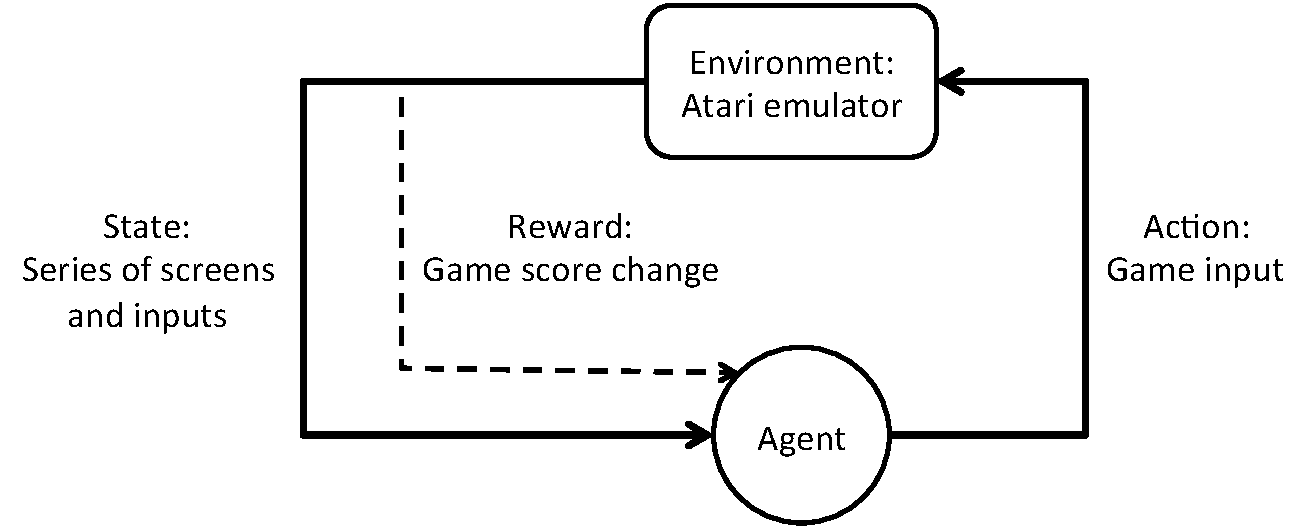
\includegraphics[width=\textwidth]{background.pdf}
    \end{figure}
\end{frame}

\begin{frame}{Playing Atari}
    \begin{itemize}\itemsep=12pt

        \item \textbf{state} sequence of game screens and inputs
        \vspace*{0.5em}
        \begin{itemize}
            \item impossible to capture current situation from only the current screen
            \item we refer to sequences and states interchangeably
        \end{itemize}

        \item \textbf{objective} learned policy maximizes discounted future rewards
        \[
            R_{t} = \sum_{t'=t}^{T} \gamma^{t'-t}r_{t'},
        \]
        with
        \vspace*{0.5em}
        \begin{itemize}
            \item game termination time step $T$
            \item discount factor $\gamma$
            \item change in reward at time $t'$ $r_{t'}$
        \end{itemize}

    \end{itemize}
\end{frame}

\begin{frame}{State-action value function}
    \begin{itemize}\itemsep=12pt
        
        \item basic idea behind RL is to estimate
        \[
            Q^{\star}\left(s, a\right) = 
            \max_{\pi}\Expect\left[R_{t} \mid s_{t} = s, a_{t} = a, \pi \right],
        \]
        where $\pi$ maps states to actions (or distributions over actions)

        \item optimal value function obeys Bellman equation
        \[
            Q^{\star}\left(s,a\right) = 
            \Expect_{s' \sim \mathcal{E}} \left[r + \gamma \max_{a'}Q^{\star}\left(s',a'\right)\mid s, a \right],
        \]
        where $\mathcal{E}$ is the MDP environment

    \end{itemize}
\end{frame}

\begin{frame}{Value approximation}
    \begin{itemize}\itemsep=12pt

        \item typically, a linear function approximator is used to estimate $Q^{\star}$
        \[
            Q\left(s,a; \theta \right) \approx Q^{\star}\left(s,a\right),
        \]
        which is parameterized by $\theta$

        \item we introduce the Q-network 
        \vspace*{0.5em}
        \begin{itemize}
            \item nonlinear neural network state-action value function approximator
            \item ``Q'' for Q-learning
        \end{itemize}

    \end{itemize}
\end{frame}

\begin{frame}{Q-network}
    \begin{itemize}\itemsep=12pt

        \item trained by minimizing a sequence of loss functions
        \[
            L_{i}\left(\theta_{i}\right) =
            \Expect_{s,a \sim \rho\left(\cdot\right)}
            \left[\left(y_{i} - Q\left(s,a;\theta_{i}\right)\right)^{2}\right],
        \]
        with
        \vspace*{0.5em}
        \begin{itemize}\itemsep=12pt
            \item iteration number $i$
            \item target $y_{i} = \Expect_{s'\sim\mathcal{E}}\left[ r + \gamma\max_{a'}Q\left(s',a';\theta_{i-1}\right) \mid s,a \right]$
            \item ``behavior distribution'' (exploration policy) $\rho\left(s,a\right)$
        \end{itemize}

        \item architecture varies according to application

    \end{itemize}
\end{frame}

\section{Algorithm}

\begin{frame}{Preprocessing}
    \begin{figure}
        \centering
        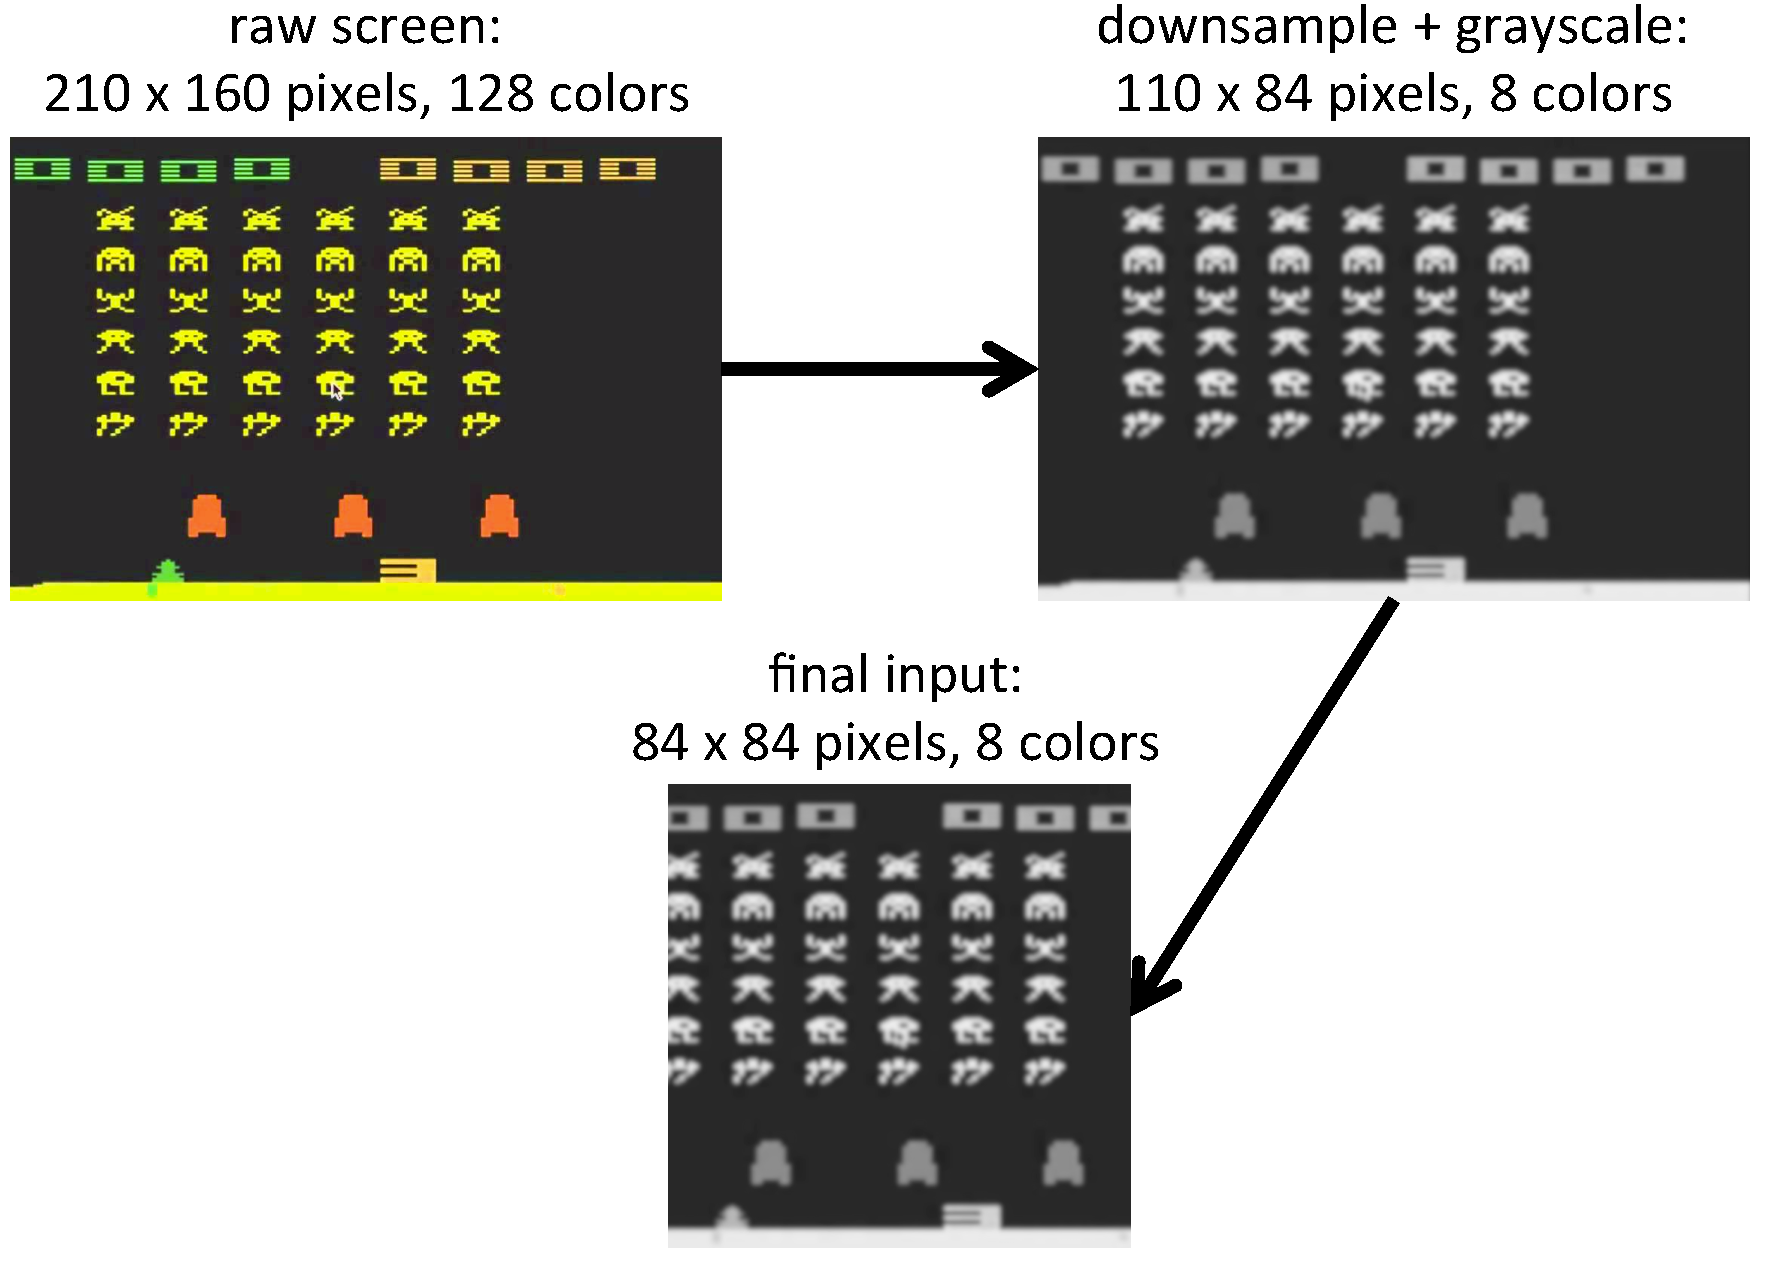
\includegraphics[width=0.9\textwidth]{process.pdf}
    \end{figure}
\end{frame}

\begin{frame}{Brief review}
    network architecture utilizes
    \vspace*{0.5em}
    \begin{itemize}\itemsep=12pt

        \item rectified nonlinearity

        \item convolutional neural network

    \end{itemize}
\end{frame}

\begin{frame}{Activation function}
    \begin{itemize}\itemsep=12pt

        \item common neural units
        \vspace*{0.5em}
        \begin{itemize}
            \item sigmoid unit 
            \[
                \frac{1}{1 + \exp\left(-x\right)}
            \]
            \item tanh unit 
            \[
                \tanh\left(x\right)
            \]
        \end{itemize}

        \item rectified nonlinearities
        \vspace*{0.5em}
        \begin{itemize}
            \item positive part (used here)
            \[
                \max\left(0,x\right) = \left(x\right)_{+}
            \]
            \item softplus
            \[
                \log\left(1 + \exp\left(x\right)\right)
            \]
        \end{itemize}

    \end{itemize}
\end{frame}

\begin{frame}{Activation function}
    \begin{figure}
        \centering
        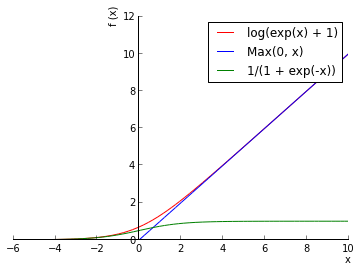
\includegraphics[width=0.7\textwidth]{neurons.png}
    \end{figure}
\end{frame}

\begin{frame}{Rectifier nonlinearity}
    \begin{itemize}\itemsep=12pt

        \item major differences
        \vspace*{0.5em}
        \begin{itemize}
            \item range of sigmoid/tanh $[0,1]$ vs. $[0,\infty]$ for rectifier units
            \item gradient of sigmoid and tanh vanishes as x increases/decreases
        \end{itemize}

        \item advantages of rectifier units \cite{JKRL:09,NH:10}
        \vspace*{0.5em}
        \begin{itemize}
            \item positive part induces sparsity in hidden units (think $\ell_{1}$-norm)
            \item no vanishing gradient problem
            \item can model real/integer valued inputs
        \end{itemize}

    \end{itemize}
\end{frame}

\begin{frame}{Convolutional neural network}
    \begin{itemize}\itemsep=12pt

        \item biologically-inspired by the visual cortex

        \item CNN example: single layer, single frame to single filter, stride = 1

    \end{itemize}
    \begin{minipage}{\textwidth}
        \centering
        \animategraphics[autoplay,loop,width=0.8\textwidth]{2}{conv-}{0}{8}
    \end{minipage}
\end{frame}

\begin{frame}{Network architecture}
    \begin{figure}
        \centering
        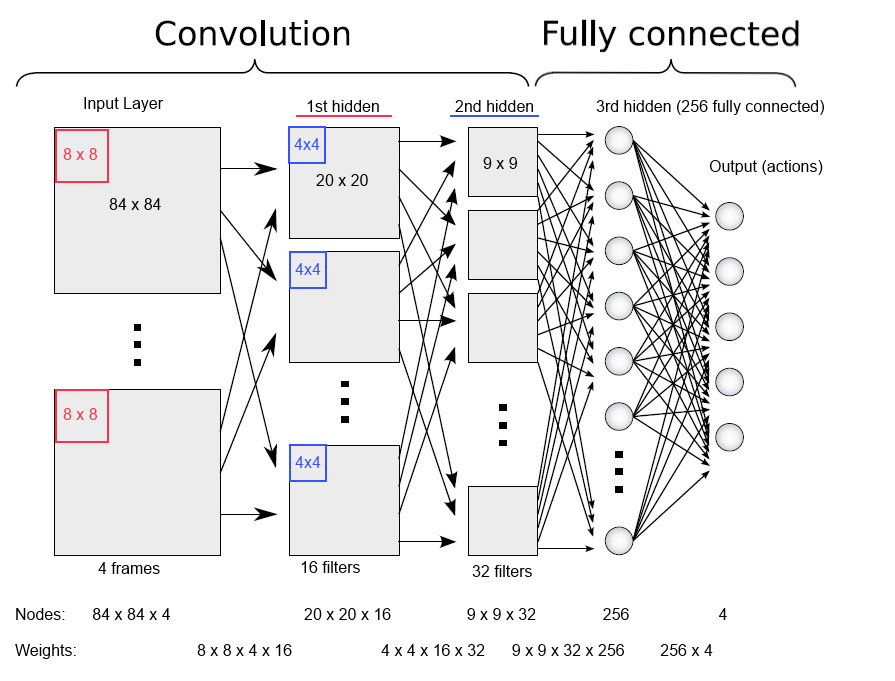
\includegraphics[width=0.9\textwidth]{neural-net.png}
    \end{figure}
\end{frame}

\begin{frame}{Stochastic gradient descent}
    \begin{itemize}\itemsep=12pt

        \item optimize Q-network loss function by gradient descent
        \[
            Q\left(s,a;\theta\right) := Q\left(s,a;\theta\right) + \alpha \nabla_{\theta} Q\left(s,a;\theta\right),
        \]
        with
        \vspace*{0.5em}
        \begin{itemize}
            \item learning rate $\alpha$
        \end{itemize}
        
        \item for computational expedience
        \vspace*{0.5em}
        \begin{itemize}
            \item update weights after every time step
            \item avoid computing full expectations
            \item replace with single samples from $\rho$ and $\mathcal{E}$
        \end{itemize}

    \end{itemize}
\end{frame}

\begin{frame}{Q-learning}
    \[
        Q\left(s,a\right) :=
        Q\left(s,a\right) +
        \alpha \left( r + \gamma\max_{a'}Q\left(s',a'\right) - Q\left(s,a\right) \right)
    \]
    \begin{itemize}\itemsep=12pt

        \item model free RL
        \vspace*{0.5em}
        \begin{itemize}
            \item avoids estimating $\mathcal{E}$
        \end{itemize}

        \item off-policy
        \vspace*{0.5em}
        \begin{itemize}
            \item learns policy $a = \argmax_{a}Q\left(s,a;\theta\right)$
            \item uses behavior distribution selected by an $\epsilon$-greedy strategy
        \end{itemize}
    
    \end{itemize}
\end{frame}

\begin{frame}{Experience replay}
    a kind of short-term memory
    \vspace*{0.5em}
    \begin{itemize}\itemsep=12pt

        \item store agent's experiences at each time step
        \[
            e_{t} = \left(s_{t},a_{t},r_{t},s_{t+1}\right)
        \]
        
        \item experiences form a replay memory dataset
        \[
            \mathcal{D} = \left\{ e_{1}, \ldots, e_{N} \right\},
        \]
        where $N$ is the fixed memory capacity

        \item execute Q-learning updates with samples of experience
        \[
            e \sim \mathcal{D}
        \]

    \end{itemize}
\end{frame}

\begin{frame}{Deep Q-learning}
    \begin{tabbing}
        {\bf given} replay memory $\mathcal{D}$ with capacity $N$ \\*[\smallskipamount]
        {\bf initialize} Q-network with random weights $\theta$ \\*[\smallskipamount]
        {\bf repeat} until timeout \\
            \qquad \= {\bf initialize} frame sequence $s_{1}=\left\{ x_{1} \right\}$ and preprocessed state $\phi_{1} = \phi\left(s_{1}\right)$ \\
            \> for \(t\) = 1, \(\ldots\) , \(T\) \\
            \qquad \qquad \= 1.\ select action $ a_{t} = \bigg\{
            \begin{tabular}{ll}
                $\max_{a}Q\left(\phi\left(s_{t}\right),a;\theta\right)$ & w.p. $1 - \epsilon$ \\
                \text{random action} & otherwise
            \end{tabular} $ \\
            \> 2.\ execute action $a_{t}$ and observe reward $r_{t}$ and frame $x_{t+1}$ \\
            \> 3.\ append $s_{t+1} = \left(s_{t}, a_{t}, x_{t+1}\right)$ and preprocess $\phi_{t+1} = \phi\left(s_{t+1}\right)$ \\
            \> 4.\ store experience $\left(\phi_{t},a_{t},r_{t},\phi_{t+1}\right)$ in $\mathcal{D}$ \\
            \> 5.\ uniformly sample minibatch $\left( \phi_{j},a_{j},r_{j},\phi_{j+1} \right) \sim \mathcal{D}$ \\
            \> 6.\ set $ y_{j} = \bigg\{
            \begin{tabular}{ll}
                $r_{j}$ & if $\phi_{j+1}$ terminal \\
                $r_{j} + \gamma\max_{a'}Q\left(\phi_{j+1},a';\theta\right)$ & otherwise
            \end{tabular} $ \\
            \> 7.\ perform gradient descent step on minibatch
    \end{tabbing}
\end{frame}

\begin{frame}{Theoretical complications}
    deep learning algorithms require
    \vspace*{0.5em}
    \begin{itemize}\itemsep=12pt

        \item huge training datasets

        \item independence between samples

        \item fixed underlying data distribution

    \end{itemize}
\end{frame}

\begin{frame}{Deep Q-learning}
    avoids theoretical complications
    \vspace*{0.5em}
    \begin{itemize}\itemsep=12pt

        \item greater data efficiency
        \vspace*{0.5em}
        \begin{itemize}
            \item each experience potentially used in many weight udpates
        \end{itemize}

        \item reduce correlations between samples
        \vspace*{0.5em}
        \begin{itemize}
            \item randomizing samples breaks correlations from consecutive samples
        \end{itemize}

        \item experience replay averages behavior distribution over states
        \vspace*{0.5em}
        \begin{itemize}
            \item smooths out learning
            \item avoids oscillations or divergence in gradient descent
        \end{itemize}

    \end{itemize}
\end{frame}

\section{Numerical experiments}

\begin{frame}{Implementation}
    \begin{itemize}\itemsep=12pt
        
        \item experiment on seven Atari 2600 games
        \vspace*{0.5em}
        \begin{itemize}
            \item Beam Rider, Breakout, Enduro, Pong, Q*bert, Seaquest, and Space Invaders
        \end{itemize}

        \item same algorithm
        \vspace*{0.5em}
        \begin{itemize}
            \item network architecture
            \item learning algorithm
            \item training hyperparameters
        \end{itemize}

        \item modified reward structure
        \vspace*{0.5em}
        \begin{itemize}
            \item all positive/negative rewards mapped to +1/$-$1
        \end{itemize}

    \end{itemize}
\end{frame}

\begin{frame}{Implementation}
    \begin{itemize}\itemsep=12pt

        \item minibatch stochastic gradient descent with RMSProp speedup
        \vspace*{0.5em}
        \begin{itemize}
            \item divide learning rate by a running average of the magnitudes of recent gradients
        \end{itemize}

        \item $\epsilon$-greedy exploration with simulated annealing 
        \vspace*{0.5em}
        \begin{itemize}
            \item linear decrease of $\epsilon$ from 1 to 0.1 for first million frames
            \item fixed value of 0.1 thereafter
        \end{itemize}

        \item experience gain with frame-skipping
        \vspace*{0.5em}
        \begin{itemize}
            \item trained for 10 million frames and memory capacity of one million
            \item observe every 4th frame (3rd for Space Invaders---because lasers!)
        \end{itemize}

    \end{itemize}
\end{frame}

\begin{frame}{Training and stability}
    \begin{itemize}\itemsep=12pt

        \item evolution of average $Q$ suggests convergence
    
    \end{itemize}
    \begin{figure}
        \centering
        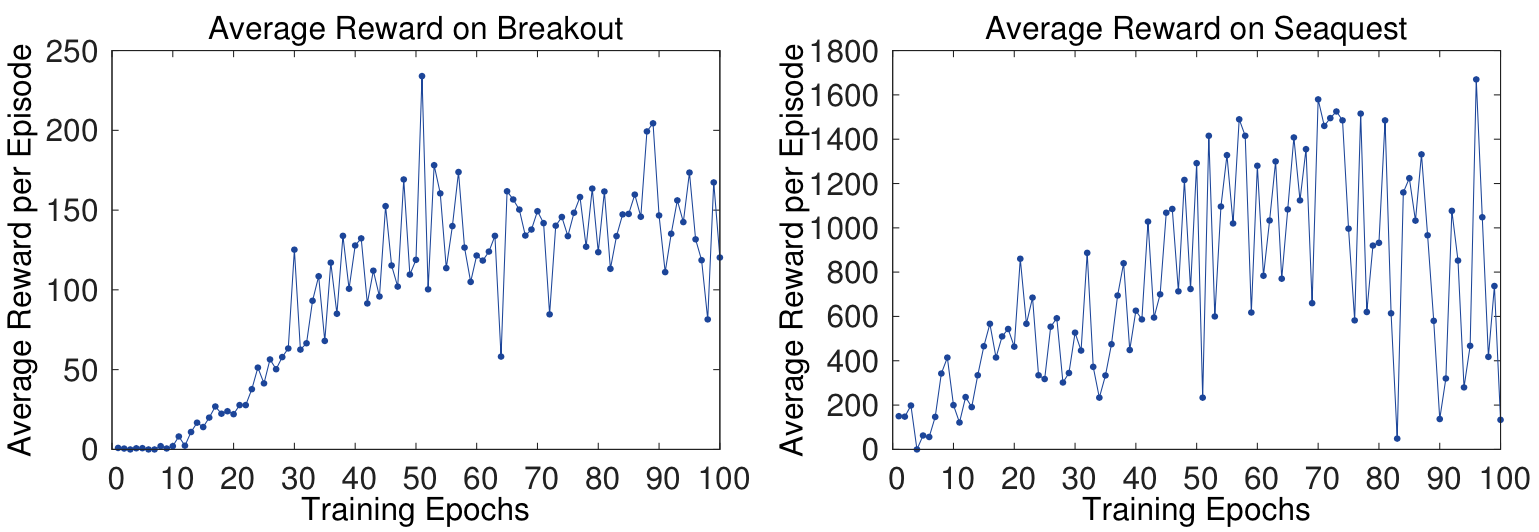
\includegraphics[width=0.8\textwidth]{stab-1.png}
    \end{figure}
    \begin{figure}
        \centering
        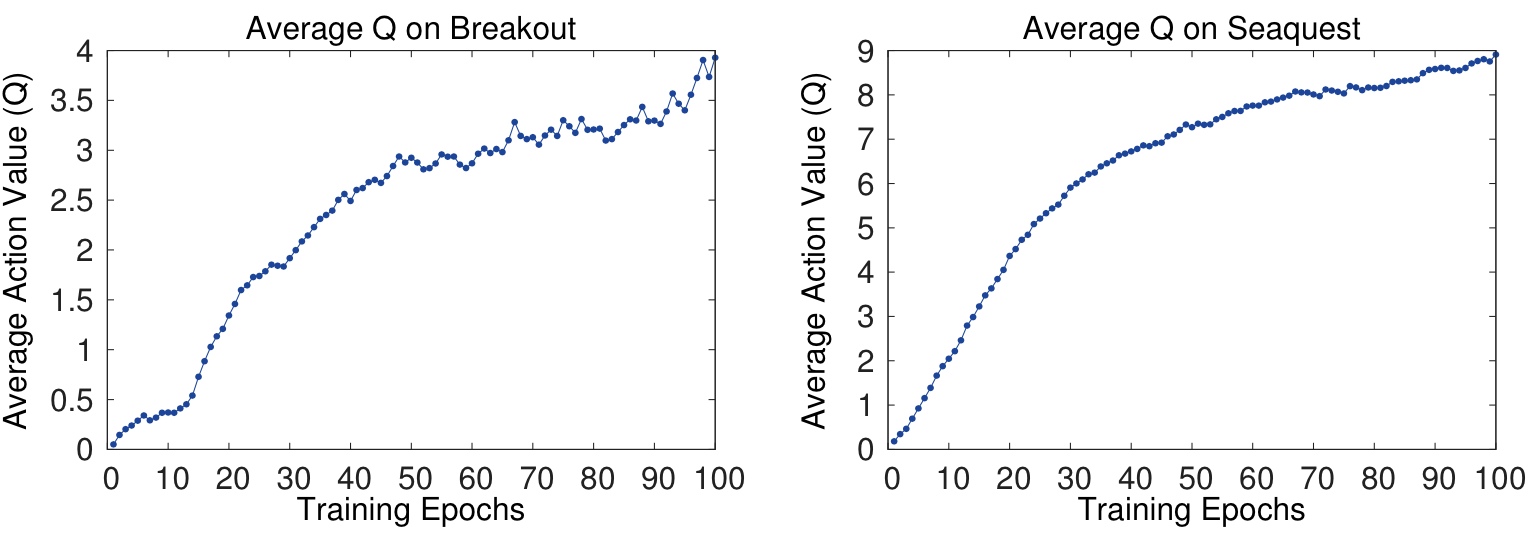
\includegraphics[width=0.8\textwidth]{stab-2.png}
    \end{figure}
\end{frame}

\begin{frame}{Visualizing the value function}
    \begin{itemize}\itemsep=12pt

        \item notice how shooting an enemy increases $Q$
    
    \end{itemize}
    \begin{figure}
        \centering
        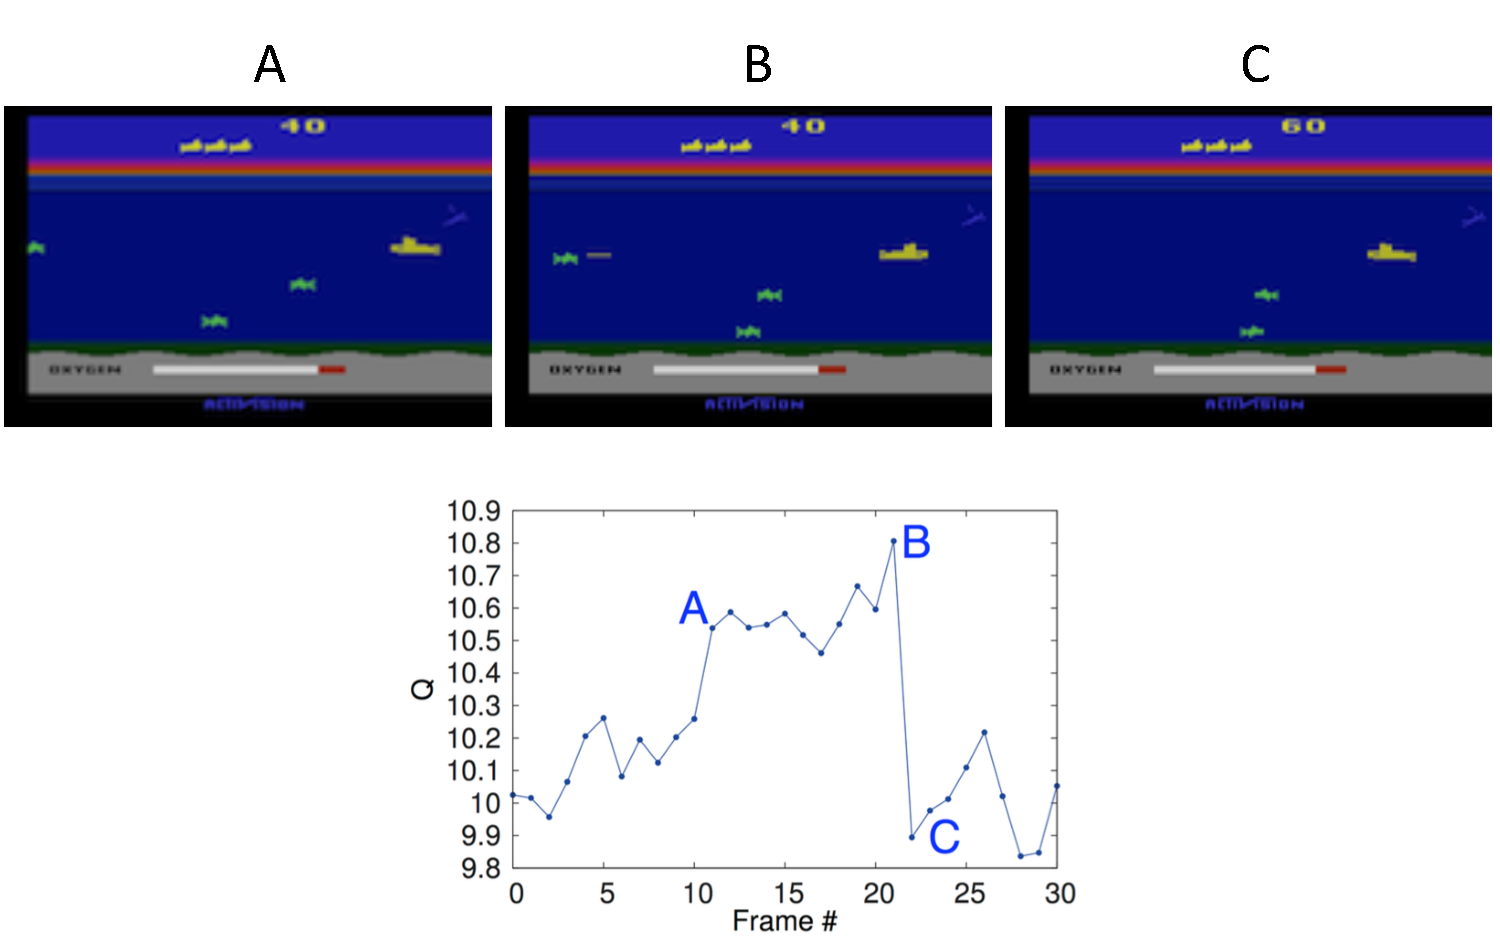
\includegraphics[width=\textwidth]{viz.pdf}
    \end{figure}
\end{frame}

\begin{frame}{Evaluation}
    \begin{itemize}\itemsep=12pt

        \item Sarsa \cite{BNVB:13}
        \vspace*{0.5em}
        \begin{itemize}
            \item Sarsa algorithm to learn linear policies
            \item uses different handcrafted feature sets for Atari games
        \end{itemize}

        \item Contingency \cite{BVB:12}
        \vspace*{0.5em}
        \begin{itemize}
            \item same basic approach as Sarsa
            \item augmented feature sets with learned representation of parts of the screen under agent's control
        \end{itemize}

        \item both approaches incorporate significant problem knowledge
        \vspace*{0.5em}
        \begin{itemize}
            \item background subtraction
            \item treating colors indicating different objects as different inputs
        \end{itemize}

    \end{itemize}
\end{frame}

\begin{frame}{Evaluation}
    HNeat \cite{SKW:13}
    \vspace*{0.5em}
    \begin{itemize}\itemsep=12pt

        \item HNeat Best uses a handcrafted object detector
        
        \item HNeat Pixel uses an 8-color channel representation of the emulator as an object label map

        \item relies heavily on finding a deterministic sequence of states that represents a successful game exploit
        \vspace*{0.5em}
        \begin{itemize}
            \item unlikely to generalize to random perturbations in general gameplay
            \item compare only against best score
        \end{itemize}

    \end{itemize}
\end{frame}

\begin{frame}{Results}
    \begin{table}[htbp!]
        \begin{minipage}{\textwidth}
            \centering
            {\scriptsize
            \begin{tabular}{lccccccc}
                \toprule
                & B. Rider & Breakout & Enduro & Pong & Q*bert & Seaquest & S. Invaders \\ \midrule
                Random & 354 & 1.2 & 0 & -20.4 & 157 & 110 & 179 \\
                Sarsa & 996 & 5.2 & 129 & -19 & 614 & 665 & 271 \\
                Contingency & 1743 & 6 & 159 & -17 & 960 & 723 & 268 \\
                DQN & 4092 & \textbf{168} & \textbf{470} & \textbf{20} & 1952 & 1705 & 581 \\
                Human & \textbf{7456} & 31 & 368 & -3 & \textbf{18900} & \textbf{28010} & \textbf{3690} \\ \midrule
                HNeat Best & 3616 & 52 & 106 & 19 & 1800 & 920 & \textbf{1720} \\
                HNeat Pixel & 1332 & 4 & 91 & -16 & 1325 & 800 & 1145 \\
                DQN Best & \textbf{5184} & \textbf{225} & \textbf{661} & \textbf{21} & \textbf{4500} & \textbf{1740} & 1075 \\
                \bottomrule
            \end{tabular}
            }
            \label{table:cluster}
        \end{minipage} 
    \end{table}
    \begin{itemize}\itemsep=12pt

        \item beat expert on Breakout, Enduro, and Pong

        \item relatively close to human performance on Beam Rider

        \item lost to expert on Q*bert, Seaquest, and Space Invaders
        \vspace*{0.5em}
        \begin{itemize}
            \item probably require strategies with long time scales
        \end{itemize}

    \end{itemize}
\end{frame}

\section{Conclusion}

\begin{frame}{Summary}
    \begin{itemize}\itemsep=12pt

        \item introduced novel deep learning model for RL

        \item demonstrated ability to master difficult game control policies with pixel input

        \item extended Q-learning with stochastic minibatch updates and experience replay

        \item \tiny{acquired by Google for \$400 million \#win \#adtech \#googleworlddomination}

    \end{itemize}
\end{frame}

\begin{frame}{Extension: prioritized sweeping}
    \begin{itemize}\itemsep=12pt

        \item uniform sampling of replay memory does not differentiate important experiences

        \item always overwrites memory with recent transitions due to finite memory size

        \item improvement could emphasize experiences from which we can learn the most with prioritized sweeping

    \end{itemize}
\end{frame}

\begin{frame}{Some issues}
    \begin{itemize}\itemsep=12pt

        \item lack of theoretical convergence guarantees

        \item lack of hardware/software implementation details

        \item lack of computational time estimates (some hints available in recorded presentation)

        \item \tiny{switching between British and American English, grammatical and spelling errors, colloquial phrases, and inconsistent figures}

    \end{itemize}
\end{frame}

\begin{frame}{Replicating DeepMind}
    \begin{itemize}\itemsep=12pt

        \item implementation attempts
        \vspace*{0.5em}
        \begin{itemize}        
            \item \url{https://github.com/kristjankorjus/Replicating-DeepMind/}
            \item \url{https://github.com/spragunr/deep\_q\_rl/}
        \end{itemize}

        \item reading list
        \vspace*{0.5em}
        \begin{itemize}
            \item \url{http://deeplearning.net/reading-list/}
        \end{itemize}

    \end{itemize}
\end{frame}

\section*{}

\begin{frame}[allowframebreaks]{References}
    \bibliography{IEEEabrv,slides}
\end{frame}

\end{document}